\documentclass[1p]{elsarticle_modified}
%\bibliographystyle{elsarticle-num}

%\usepackage[colorlinks]{hyperref}
%\usepackage{abbrmath_seonhwa} %\Abb, \Ascr, \Acal ,\Abf, \Afrak
\usepackage{amsfonts}
\usepackage{amssymb}
\usepackage{amsmath}
\usepackage{amsthm}
\usepackage{scalefnt}
\usepackage{amsbsy}
\usepackage{kotex}
\usepackage{caption}
\usepackage{subfig}
\usepackage{color}
\usepackage{graphicx}
\usepackage{xcolor} %% white, black, red, green, blue, cyan, magenta, yellow
\usepackage{float}
\usepackage{setspace}
\usepackage{hyperref}

\usepackage{tikz}
\usetikzlibrary{arrows}

\usepackage{multirow}
\usepackage{array} % fixed length table
\usepackage{hhline}

%%%%%%%%%%%%%%%%%%%%%
\makeatletter
\renewcommand*\env@matrix[1][\arraystretch]{%
	\edef\arraystretch{#1}%
	\hskip -\arraycolsep
	\let\@ifnextchar\new@ifnextchar
	\array{*\c@MaxMatrixCols c}}
\makeatother %https://tex.stackexchange.com/questions/14071/how-can-i-increase-the-line-spacing-in-a-matrix
%%%%%%%%%%%%%%%

\usepackage[normalem]{ulem}

\newcommand{\msout}[1]{\ifmmode\text{\sout{\ensuremath{#1}}}\else\sout{#1}\fi}
%SOURCE: \msout is \stkout macro in https://tex.stackexchange.com/questions/20609/strikeout-in-math-mode

\newcommand{\cancel}[1]{
	\ifmmode
	{\color{red}\msout{#1}}
	\else
	{\color{red}\sout{#1}}
	\fi
}

\newcommand{\add}[1]{
	{\color{blue}\uwave{#1}}
}

\newcommand{\replace}[2]{
	\ifmmode
	{\color{red}\msout{#1}}{\color{blue}\uwave{#2}}
	\else
	{\color{red}\sout{#1}}{\color{blue}\uwave{#2}}
	\fi
}

\newcommand{\Sol}{\mathcal{S}} %segment
\newcommand{\D}{D} %diagram
\newcommand{\A}{\mathcal{A}} %arc


%%%%%%%%%%%%%%%%%%%%%%%%%%%%%5 test

\def\sl{\operatorname{\textup{SL}}(2,\Cbb)}
\def\psl{\operatorname{\textup{PSL}}(2,\Cbb)}
\def\quan{\mkern 1mu \triangleright \mkern 1mu}

\theoremstyle{definition}
\newtheorem{thm}{Theorem}[section]
\newtheorem{prop}[thm]{Proposition}
\newtheorem{lem}[thm]{Lemma}
\newtheorem{ques}[thm]{Question}
\newtheorem{cor}[thm]{Corollary}
\newtheorem{defn}[thm]{Definition}
\newtheorem{exam}[thm]{Example}
\newtheorem{rmk}[thm]{Remark}
\newtheorem{alg}[thm]{Algorithm}

\newcommand{\I}{\sqrt{-1}}
\begin{document}

%\begin{frontmatter}
%
%\title{Boundary parabolic representations of knots up to 8 crossings}
%
%%% Group authors per affiliation:
%\author{Yunhi Cho} 
%\address{Department of Mathematics, University of Seoul, Seoul, Korea}
%\ead{yhcho@uos.ac.kr}
%
%
%\author{Seonhwa Kim} %\fnref{s_kim}}
%\address{Center for Geometry and Physics, Institute for Basic Science, Pohang, 37673, Korea}
%\ead{ryeona17@ibs.re.kr}
%
%\author{Hyuk Kim}
%\address{Department of Mathematical Sciences, Seoul National University, Seoul 08826, Korea}
%\ead{hyukkim@snu.ac.kr}
%
%\author{Seokbeom Yoon}
%\address{Department of Mathematical Sciences, Seoul National University, Seoul, 08826,  Korea}
%\ead{sbyoon15@snu.ac.kr}
%
%\begin{abstract}
%We find all boundary parabolic representation of knots up to 8 crossings.
%
%\end{abstract}
%\begin{keyword}
%    \MSC[2010] 57M25 
%\end{keyword}
%
%\end{frontmatter}

%\linenumbers
%\tableofcontents
%
\newcommand\colored[1]{\textcolor{white}{\rule[-0.35ex]{0.8em}{1.4ex}}\kern-0.8em\color{red} #1}%
%\newcommand\colored[1]{\textcolor{white}{ #1}\kern-2.17ex	\textcolor{white}{ #1}\kern-1.81ex	\textcolor{white}{ #1}\kern-2.15ex\color{red}#1	}

{\Large $\underline{12n_{0855}~(K12n_{0855})}$}

\setlength{\tabcolsep}{10pt}
\renewcommand{\arraystretch}{1.6}
\vspace{1cm}\begin{tabular}{m{100pt}>{\centering\arraybackslash}m{274pt}}
\multirow{5}{120pt}{
	\centering
	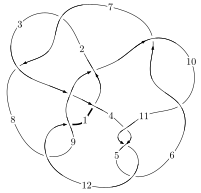
\includegraphics[width=112pt]{../../../GIT/diagram.site/Diagrams/png/2944_12n_0855.png}\\
\ \ \ A knot diagram\footnotemark}&
\allowdisplaybreaks
\textbf{Linearized knot diagam} \\
\cline{2-2}
 &
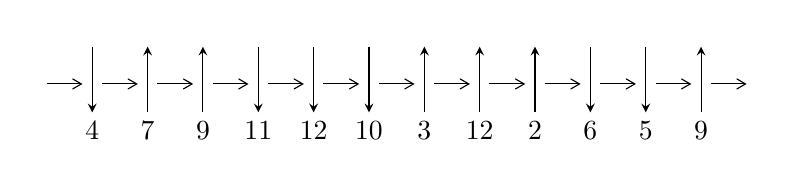
\begin{tikzpicture}[x=20pt, y=17pt]
	% nodes
	\node (C0) at (0, 0) {};
	\node (C1) at (1, 0) {};
	\node (C1U) at (1, +1) {};
	\node (C1D) at (1, -1) {4};

	\node (C2) at (2, 0) {};
	\node (C2U) at (2, +1) {};
	\node (C2D) at (2, -1) {7};

	\node (C3) at (3, 0) {};
	\node (C3U) at (3, +1) {};
	\node (C3D) at (3, -1) {9};

	\node (C4) at (4, 0) {};
	\node (C4U) at (4, +1) {};
	\node (C4D) at (4, -1) {11};

	\node (C5) at (5, 0) {};
	\node (C5U) at (5, +1) {};
	\node (C5D) at (5, -1) {12};

	\node (C6) at (6, 0) {};
	\node (C6U) at (6, +1) {};
	\node (C6D) at (6, -1) {10};

	\node (C7) at (7, 0) {};
	\node (C7U) at (7, +1) {};
	\node (C7D) at (7, -1) {3};

	\node (C8) at (8, 0) {};
	\node (C8U) at (8, +1) {};
	\node (C8D) at (8, -1) {12};

	\node (C9) at (9, 0) {};
	\node (C9U) at (9, +1) {};
	\node (C9D) at (9, -1) {2};

	\node (C10) at (10, 0) {};
	\node (C10U) at (10, +1) {};
	\node (C10D) at (10, -1) {6};

	\node (C11) at (11, 0) {};
	\node (C11U) at (11, +1) {};
	\node (C11D) at (11, -1) {5};

	\node (C12) at (12, 0) {};
	\node (C12U) at (12, +1) {};
	\node (C12D) at (12, -1) {9};
	\node (C13) at (13, 0) {};

	% arrows
	\draw[->,>={angle 60}]
	(C0) edge (C1) (C1) edge (C2) (C2) edge (C3) (C3) edge (C4) (C4) edge (C5) (C5) edge (C6) (C6) edge (C7) (C7) edge (C8) (C8) edge (C9) (C9) edge (C10) (C10) edge (C11) (C11) edge (C12) (C12) edge (C13) ;	\draw[->,>=stealth]
	(C1U) edge (C1D) (C2D) edge (C2U) (C3D) edge (C3U) (C4U) edge (C4D) (C5U) edge (C5D) (C6U) edge (C6D) (C7D) edge (C7U) (C8D) edge (C8U) (C9D) edge (C9U) (C10U) edge (C10D) (C11U) edge (C11D) (C12D) edge (C12U) ;
	\end{tikzpicture} \\
\hhline{~~} \\& 
\textbf{Solving Sequence} \\ \cline{2-2} 
 &
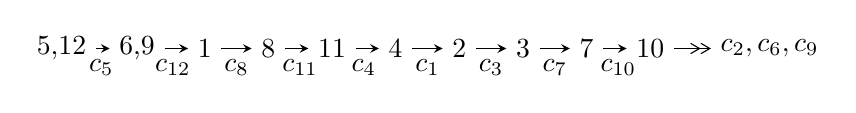
\begin{tikzpicture}[x=23pt, y=7pt]
	% node
	\node (A0) at (-1/8, 0) {5,12};
	\node (A1) at (17/16, 0) {6,9};
	\node (A2) at (17/8, 0) {1};
	\node (A3) at (25/8, 0) {8};
	\node (A4) at (33/8, 0) {11};
	\node (A5) at (41/8, 0) {4};
	\node (A6) at (49/8, 0) {2};
	\node (A7) at (57/8, 0) {3};
	\node (A8) at (65/8, 0) {7};
	\node (A9) at (73/8, 0) {10};
	\node (C1) at (1/2, -1) {$c_{5}$};
	\node (C2) at (13/8, -1) {$c_{12}$};
	\node (C3) at (21/8, -1) {$c_{8}$};
	\node (C4) at (29/8, -1) {$c_{11}$};
	\node (C5) at (37/8, -1) {$c_{4}$};
	\node (C6) at (45/8, -1) {$c_{1}$};
	\node (C7) at (53/8, -1) {$c_{3}$};
	\node (C8) at (61/8, -1) {$c_{7}$};
	\node (C9) at (69/8, -1) {$c_{10}$};
	\node (A10) at (11, 0) {$c_{2},c_{6},c_{9}$};

	% edge
	\draw[->,>=stealth]	
	(A0) edge (A1) (A1) edge (A2) (A2) edge (A3) (A3) edge (A4) (A4) edge (A5) (A5) edge (A6) (A6) edge (A7) (A7) edge (A8) (A8) edge (A9) ;
	\draw[->>,>={angle 60}]	
	(A9) edge (A10);
\end{tikzpicture} \\ 

\end{tabular} \\

\footnotetext{
The image of knot diagram is generated by the software ``\textbf{Draw programme}" developed by Andrew Bartholomew(\url{http://www.layer8.co.uk/maths/draw/index.htm\#Running-draw}), where we modified some parts for our purpose(\url{https://github.com/CATsTAILs/LinksPainter}).
}\phantom \\ \newline 
\centering \textbf{Ideals for irreducible components\footnotemark of $X_{\text{par}}$} 
 
\begin{align*}
I^u_{1}&=\langle 
-5 u^{24}-19 u^{23}+\cdots+2 b+18,\;- u^{24}-3 u^{23}+\cdots+4 a+4,\;u^{25}+5 u^{24}+\cdots+10 u-4\rangle \\
I^u_{2}&=\langle 
20 u^7 a^3-10 u^7 a^2+\cdots-62 a+47,\;-3 u^7 a^2+6 u^7 a+\cdots-20 a-11,\;u^8- u^7-3 u^6+2 u^5+3 u^4-2 u-1\rangle \\
I^u_{3}&=\langle 
u^{14}- u^{13}-5 u^{12}+5 u^{11}+8 u^{10}-8 u^9- u^8+u^7-8 u^6+8 u^5+3 u^4-4 u^3+4 u^2+b-3 u,\\
\phantom{I^u_{3}}&\phantom{= \langle  }u^{14}-6 u^{12}+13 u^{10}-9 u^8-7 u^6+11 u^4- u^3+a+u-3,\\
\phantom{I^u_{3}}&\phantom{= \langle  }u^{15}-7 u^{13}+19 u^{11}-22 u^9+3 u^7+14 u^5- u^4-6 u^3+2 u^2-3 u-1\rangle \\
\\
\end{align*}
\raggedright * 3 irreducible components of $\dim_{\mathbb{C}}=0$, with total 72 representations.\\
\footnotetext{All coefficients of polynomials are rational numbers. But the coefficients are sometimes approximated in decimal forms when there is not enough margin.}
\newpage
\renewcommand{\arraystretch}{1}
\centering \section*{I. $I^u_{1}= \langle -5 u^{24}-19 u^{23}+\cdots+2 b+18,\;- u^{24}-3 u^{23}+\cdots+4 a+4,\;u^{25}+5 u^{24}+\cdots+10 u-4 \rangle$}
\flushleft \textbf{(i) Arc colorings}\\
\begin{tabular}{m{7pt} m{180pt} m{7pt} m{180pt} }
\flushright $a_{5}=$&$\begin{pmatrix}1\\0\end{pmatrix}$ \\
\flushright $a_{12}=$&$\begin{pmatrix}0\\u\end{pmatrix}$ \\
\flushright $a_{6}=$&$\begin{pmatrix}1\\u^2\end{pmatrix}$ \\
\flushright $a_{9}=$&$\begin{pmatrix}\frac{1}{4} u^{24}+\frac{3}{4} u^{23}+\cdots+\frac{25}{4} u-1\\\frac{5}{2} u^{24}+\frac{19}{2} u^{23}+\cdots+\frac{61}{2} u-9\end{pmatrix}$ \\
\flushright $a_{1}=$&$\begin{pmatrix}-7 u^{24}-\frac{51}{2} u^{23}+\cdots-\frac{131}{2} u+\frac{41}{2}\\-\frac{45}{2} u^{24}-\frac{161}{2} u^{23}+\cdots-\frac{391}{2} u+62\end{pmatrix}$ \\
\flushright $a_{8}=$&$\begin{pmatrix}\frac{1}{4} u^{24}+\frac{3}{4} u^{23}+\cdots+\frac{25}{4} u-1\\\frac{7}{2} u^{24}+\frac{25}{2} u^{23}+\cdots+\frac{73}{2} u-11\end{pmatrix}$ \\
\flushright $a_{11}=$&$\begin{pmatrix}u\\u\end{pmatrix}$ \\
\flushright $a_{4}=$&$\begin{pmatrix}- u^2+1\\- u^2\end{pmatrix}$ \\
\flushright $a_{2}=$&$\begin{pmatrix}\frac{1}{2} u^{24}+3 u^{23}+\cdots+11 u-\frac{7}{2}\\-\frac{11}{2} u^{24}-\frac{35}{2} u^{23}+\cdots-\frac{55}{2} u+10\end{pmatrix}$ \\
\flushright $a_{3}=$&$\begin{pmatrix}-7 u^{24}-\frac{51}{2} u^{23}+\cdots-\frac{131}{2} u+\frac{43}{2}\\-\frac{45}{2} u^{24}-\frac{161}{2} u^{23}+\cdots-\frac{393}{2} u+62\end{pmatrix}$ \\
\flushright $a_{7}=$&$\begin{pmatrix}u^6-3 u^4+2 u^2+1\\u^8-2 u^6+2 u^2\end{pmatrix}$ \\
\flushright $a_{10}=$&$\begin{pmatrix}- u^3+2 u\\- u^5+u^3+u\end{pmatrix}$\\&\end{tabular}
\flushleft \textbf{(ii) Obstruction class $= -1$}\\~\\
\flushleft \textbf{(iii) Cusp Shapes $= 11 u^{24}+41 u^{23}-32 u^{22}-241 u^{21}+37 u^{20}+663 u^{19}-146 u^{18}-999 u^{17}+733 u^{16}+604 u^{15}-1604 u^{14}+758 u^{13}+1393 u^{12}-2013 u^{11}+411 u^{10}+1454 u^9-1775 u^8+369 u^7+901 u^6-1088 u^5+350 u^4+208 u^3-373 u^2+164 u-46$}\\~\\
\newpage\renewcommand{\arraystretch}{1}
\flushleft \textbf{(iv) u-Polynomials at the component}\newline \\
\begin{tabular}{m{50pt}|m{274pt}}
Crossings & \hspace{64pt}u-Polynomials at each crossing \\
\hline $$\begin{aligned}c_{1}\end{aligned}$$&$\begin{aligned}
&u^{25}-21 u^{24}+\cdots+1792 u-256
\end{aligned}$\\
\hline $$\begin{aligned}c_{2},c_{7},c_{9}\end{aligned}$$&$\begin{aligned}
&u^{25}+u^{24}+\cdots+u+1
\end{aligned}$\\
\hline $$\begin{aligned}c_{3},c_{8},c_{12}\end{aligned}$$&$\begin{aligned}
&u^{25}+18 u^{23}+\cdots+20 u^2+1
\end{aligned}$\\
\hline $$\begin{aligned}c_{4},c_{5},c_{11}\end{aligned}$$&$\begin{aligned}
&u^{25}-5 u^{24}+\cdots+10 u+4
\end{aligned}$\\
\hline $$\begin{aligned}c_{6},c_{10}\end{aligned}$$&$\begin{aligned}
&u^{25}+15 u^{24}+\cdots-1986 u-196
\end{aligned}$\\
\hline
\end{tabular}\\~\\
\newpage\renewcommand{\arraystretch}{1}
\flushleft \textbf{(v) Riley Polynomials at the component}\newline \\
\begin{tabular}{m{50pt}|m{274pt}}
Crossings & \hspace{64pt}Riley Polynomials at each crossing \\
\hline $$\begin{aligned}c_{1}\end{aligned}$$&$\begin{aligned}
&y^{25}-13 y^{24}+\cdots-131072 y-65536
\end{aligned}$\\
\hline $$\begin{aligned}c_{2},c_{7},c_{9}\end{aligned}$$&$\begin{aligned}
&y^{25}-15 y^{24}+\cdots+9 y-1
\end{aligned}$\\
\hline $$\begin{aligned}c_{3},c_{8},c_{12}\end{aligned}$$&$\begin{aligned}
&y^{25}+36 y^{24}+\cdots-40 y-1
\end{aligned}$\\
\hline $$\begin{aligned}c_{4},c_{5},c_{11}\end{aligned}$$&$\begin{aligned}
&y^{25}-21 y^{24}+\cdots-100 y-16
\end{aligned}$\\
\hline $$\begin{aligned}c_{6},c_{10}\end{aligned}$$&$\begin{aligned}
&y^{25}+15 y^{24}+\cdots-132996 y-38416
\end{aligned}$\\
\hline
\end{tabular}\\~\\
\newpage\flushleft \textbf{(vi) Complex Volumes and Cusp Shapes}
$$\begin{array}{c|c|c}  
\text{Solutions to }I^u_{1}& \I (\text{vol} + \sqrt{-1}CS) & \text{Cusp shape}\\
 \hline 
\begin{aligned}
u &= \phantom{-}0.042442 + 0.868462 I \\
a &= -0.716248 + 0.009860 I \\
b &= -0.315314 - 0.333618 I\end{aligned}
 & \phantom{-}6.65854 - 2.22451 I & \phantom{-}1.85427 + 3.24248 I \\ \hline\begin{aligned}
u &= \phantom{-}0.042442 - 0.868462 I \\
a &= -0.716248 - 0.009860 I \\
b &= -0.315314 + 0.333618 I\end{aligned}
 & \phantom{-}6.65854 + 2.22451 I & \phantom{-}1.85427 - 3.24248 I \\ \hline\begin{aligned}
u &= \phantom{-}0.170420 + 0.851806 I \\
a &= -1.68479 - 1.05733 I \\
b &= -0.313941 - 1.151630 I\end{aligned}
 & \phantom{-}1.36106 - 10.21960 I & \phantom{-}3.12273 + 6.18876 I \\ \hline\begin{aligned}
u &= \phantom{-}0.170420 - 0.851806 I \\
a &= -1.68479 + 1.05733 I \\
b &= -0.313941 + 1.151630 I\end{aligned}
 & \phantom{-}1.36106 + 10.21960 I & \phantom{-}3.12273 - 6.18876 I \\ \hline\begin{aligned}
u &= \phantom{-}0.689863 + 0.516195 I \\
a &= \phantom{-}0.90028 + 1.54729 I \\
b &= \phantom{-}0.157173 + 0.858656 I\end{aligned}
 & -2.89781 - 4.73922 I & \phantom{-}0.64335 + 6.01647 I \\ \hline\begin{aligned}
u &= \phantom{-}0.689863 - 0.516195 I \\
a &= \phantom{-}0.90028 - 1.54729 I \\
b &= \phantom{-}0.157173 - 0.858656 I\end{aligned}
 & -2.89781 + 4.73922 I & \phantom{-}0.64335 - 6.01647 I \\ \hline\begin{aligned}
u &= \phantom{-}1.062620 + 0.439244 I \\
a &= -0.93017 - 1.06985 I \\
b &= -0.393102 - 0.665533 I\end{aligned}
 & -1.37637 + 5.59077 I & \phantom{-}0.49701 - 2.52369 I \\ \hline\begin{aligned}
u &= \phantom{-}1.062620 - 0.439244 I \\
a &= -0.93017 + 1.06985 I \\
b &= -0.393102 + 0.665533 I\end{aligned}
 & -1.37637 - 5.59077 I & \phantom{-}0.49701 + 2.52369 I \\ \hline\begin{aligned}
u &= \phantom{-}0.370519 + 0.720063 I \\
a &= \phantom{-}1.56474 + 0.89351 I \\
b &= \phantom{-}0.401573 + 0.852679 I\end{aligned}
 & -1.86125 + 0.38147 I & \phantom{-}3.19263 - 0.66430 I \\ \hline\begin{aligned}
u &= \phantom{-}0.370519 - 0.720063 I \\
a &= \phantom{-}1.56474 - 0.89351 I \\
b &= \phantom{-}0.401573 - 0.852679 I\end{aligned}
 & -1.86125 - 0.38147 I & \phantom{-}3.19263 + 0.66430 I\\
 \hline 
 \end{array}$$\newpage$$\begin{array}{c|c|c}  
\text{Solutions to }I^u_{1}& \I (\text{vol} + \sqrt{-1}CS) & \text{Cusp shape}\\
 \hline 
\begin{aligned}
u &= \phantom{-}1.27648\phantom{ +0.000000I} \\
a &= \phantom{-}0.500312\phantom{ +0.000000I} \\
b &= \phantom{-}0.280537\phantom{ +0.000000I}\end{aligned}
 & -2.96177\phantom{ +0.000000I} & -0.698220\phantom{ +0.000000I} \\ \hline\begin{aligned}
u &= -1.296580 + 0.136250 I \\
a &= \phantom{-}0.004316 - 0.323358 I \\
b &= \phantom{-}0.429924 - 1.218120 I\end{aligned}
 & -4.47329 + 2.69307 I & -5.03326 - 5.98784 I \\ \hline\begin{aligned}
u &= -1.296580 - 0.136250 I \\
a &= \phantom{-}0.004316 + 0.323358 I \\
b &= \phantom{-}0.429924 + 1.218120 I\end{aligned}
 & -4.47329 - 2.69307 I & -5.03326 + 5.98784 I \\ \hline\begin{aligned}
u &= \phantom{-}1.235760 + 0.416433 I \\
a &= -0.139402 - 0.504528 I \\
b &= -0.038519 - 0.297655 I\end{aligned}
 & \phantom{-}2.97397 - 2.37583 I & -1.057681 + 0.915229 I \\ \hline\begin{aligned}
u &= \phantom{-}1.235760 - 0.416433 I \\
a &= -0.139402 + 0.504528 I \\
b &= -0.038519 + 0.297655 I\end{aligned}
 & \phantom{-}2.97397 + 2.37583 I & -1.057681 - 0.915229 I \\ \hline\begin{aligned}
u &= -1.304980 + 0.396966 I \\
a &= -0.149198 + 0.398993 I \\
b &= -0.962816 + 0.648234 I\end{aligned}
 & \phantom{-}2.45389 + 6.76060 I & -2.28268 - 6.77573 I \\ \hline\begin{aligned}
u &= -1.304980 - 0.396966 I \\
a &= -0.149198 - 0.398993 I \\
b &= -0.962816 - 0.648234 I\end{aligned}
 & \phantom{-}2.45389 - 6.76060 I & -2.28268 + 6.77573 I \\ \hline\begin{aligned}
u &= -1.37760 + 0.36657 I \\
a &= \phantom{-}0.142768 + 1.259210 I \\
b &= -1.32923 + 3.16497 I\end{aligned}
 & -3.5266 + 14.6054 I & -1.02784 - 7.76061 I \\ \hline\begin{aligned}
u &= -1.37760 - 0.36657 I \\
a &= \phantom{-}0.142768 - 1.259210 I \\
b &= -1.32923 - 3.16497 I\end{aligned}
 & -3.5266 - 14.6054 I & -1.02784 + 7.76061 I \\ \hline\begin{aligned}
u &= -1.44314 + 0.25974 I \\
a &= \phantom{-}0.006895 - 1.095370 I \\
b &= \phantom{-}1.09681 - 2.92836 I\end{aligned}
 & -7.68655 + 3.14182 I & \phantom{-}0.46512 + 1.43904 I\\
 \hline 
 \end{array}$$\newpage$$\begin{array}{c|c|c}  
\text{Solutions to }I^u_{1}& \I (\text{vol} + \sqrt{-1}CS) & \text{Cusp shape}\\
 \hline 
\begin{aligned}
u &= -1.44314 - 0.25974 I \\
a &= \phantom{-}0.006895 + 1.095370 I \\
b &= \phantom{-}1.09681 + 2.92836 I\end{aligned}
 & -7.68655 - 3.14182 I & \phantom{-}0.46512 - 1.43904 I \\ \hline\begin{aligned}
u &= -1.46408 + 0.08648 I \\
a &= -0.108140 - 1.228800 I \\
b &= \phantom{-}0.14349 - 3.82971 I\end{aligned}
 & -9.92989 + 6.47027 I & -4.20740 - 5.48144 I \\ \hline\begin{aligned}
u &= -1.46408 - 0.08648 I \\
a &= -0.108140 + 1.228800 I \\
b &= \phantom{-}0.14349 + 3.82971 I\end{aligned}
 & -9.92989 - 6.47027 I & -4.20740 + 5.48144 I \\ \hline\begin{aligned}
u &= \phantom{-}0.176540 + 0.371053 I \\
a &= \phantom{-}0.608793 + 0.633615 I \\
b &= -0.016319 + 0.292219 I\end{aligned}
 & \phantom{-}0.045964 - 0.832254 I & \phantom{-}1.18286 + 8.33998 I \\ \hline\begin{aligned}
u &= \phantom{-}0.176540 - 0.371053 I \\
a &= \phantom{-}0.608793 - 0.633615 I \\
b &= -0.016319 - 0.292219 I\end{aligned}
 & \phantom{-}0.045964 + 0.832254 I & \phantom{-}1.18286 - 8.33998 I\\
 \hline 
 \end{array}$$\newpage\newpage\renewcommand{\arraystretch}{1}
\centering \section*{II. $I^u_{2}= \langle 20 u^7 a^3-10 u^7 a^2+\cdots-62 a+47,\;-3 u^7 a^2+6 u^7 a+\cdots-20 a-11,\;u^8- u^7-3 u^6+2 u^5+3 u^4-2 u-1 \rangle$}
\flushleft \textbf{(i) Arc colorings}\\
\begin{tabular}{m{7pt} m{180pt} m{7pt} m{180pt} }
\flushright $a_{5}=$&$\begin{pmatrix}1\\0\end{pmatrix}$ \\
\flushright $a_{12}=$&$\begin{pmatrix}0\\u\end{pmatrix}$ \\
\flushright $a_{6}=$&$\begin{pmatrix}1\\u^2\end{pmatrix}$ \\
\flushright $a_{9}=$&$\begin{pmatrix}a\\-0.465116 a^{3} u^{7}+0.232558 a^{2} u^{7}+\cdots+1.44186 a-1.09302\end{pmatrix}$ \\
\flushright $a_{1}=$&$\begin{pmatrix}a^2 u\\-0.790698 a^{3} u^{7}+1.39535 a^{2} u^{7}+\cdots+0.651163 a-0.558140\end{pmatrix}$ \\
\flushright $a_{8}=$&$\begin{pmatrix}a\\-0.465116 a^{3} u^{7}+0.232558 a^{2} u^{7}+\cdots+1.44186 a-1.09302\end{pmatrix}$ \\
\flushright $a_{11}=$&$\begin{pmatrix}u\\u\end{pmatrix}$ \\
\flushright $a_{4}=$&$\begin{pmatrix}- u^2+1\\- u^2\end{pmatrix}$ \\
\flushright $a_{2}=$&$\begin{pmatrix}0.116279 a^{3} u^{7}+0.441860 a^{2} u^{7}+\cdots+0.139535 a+1.02326\\-0.302326 a^{3} u^{7}+1.65116 a^{2} u^{7}+\cdots+0.837209 a+0.139535\end{pmatrix}$ \\
\flushright $a_{3}=$&$\begin{pmatrix}0.186047 a^{3} u^{7}-0.0930233 a^{2} u^{7}+\cdots+0.0232558 a+0.837209\\1.90698 a^{3} u^{7}-1.95349 a^{2} u^{7}+\cdots-0.511628 a-0.418605\end{pmatrix}$ \\
\flushright $a_{7}=$&$\begin{pmatrix}u^6-3 u^4+2 u^2+1\\u^7+u^6-2 u^5-3 u^4+2 u^2+2 u+1\end{pmatrix}$ \\
\flushright $a_{10}=$&$\begin{pmatrix}- u^3+2 u\\- u^5+u^3+u\end{pmatrix}$\\&\end{tabular}
\flushleft \textbf{(ii) Obstruction class $= -1$}\\~\\
\flushleft \textbf{(iii) Cusp Shapes $= -4 u^6+12 u^4+4 u^3-8 u^2-8 u-6$}\\~\\
\newpage\renewcommand{\arraystretch}{1}
\flushleft \textbf{(iv) u-Polynomials at the component}\newline \\
\begin{tabular}{m{50pt}|m{274pt}}
Crossings & \hspace{64pt}u-Polynomials at each crossing \\
\hline $$\begin{aligned}c_{1}\end{aligned}$$&$\begin{aligned}
&(u^2+u-1)^{16}
\end{aligned}$\\
\hline $$\begin{aligned}c_{2},c_{7},c_{9}\end{aligned}$$&$\begin{aligned}
&u^{32}+u^{31}+\cdots+318 u+199
\end{aligned}$\\
\hline $$\begin{aligned}c_{3},c_{8},c_{12}\end{aligned}$$&$\begin{aligned}
&u^{32}- u^{31}+\cdots-1792 u-271
\end{aligned}$\\
\hline $$\begin{aligned}c_{4},c_{5},c_{11}\end{aligned}$$&$\begin{aligned}
&(u^8+u^7-3 u^6-2 u^5+3 u^4+2 u-1)^4
\end{aligned}$\\
\hline $$\begin{aligned}c_{6},c_{10}\end{aligned}$$&$\begin{aligned}
&(u^8-3 u^7+7 u^6-10 u^5+11 u^4-10 u^3+6 u^2-4 u+1)^4
\end{aligned}$\\
\hline
\end{tabular}\\~\\
\newpage\renewcommand{\arraystretch}{1}
\flushleft \textbf{(v) Riley Polynomials at the component}\newline \\
\begin{tabular}{m{50pt}|m{274pt}}
Crossings & \hspace{64pt}Riley Polynomials at each crossing \\
\hline $$\begin{aligned}c_{1}\end{aligned}$$&$\begin{aligned}
&(y^2-3 y+1)^{16}
\end{aligned}$\\
\hline $$\begin{aligned}c_{2},c_{7},c_{9}\end{aligned}$$&$\begin{aligned}
&y^{32}-13 y^{31}+\cdots-651956 y+39601
\end{aligned}$\\
\hline $$\begin{aligned}c_{3},c_{8},c_{12}\end{aligned}$$&$\begin{aligned}
&y^{32}+19 y^{31}+\cdots-1289332 y+73441
\end{aligned}$\\
\hline $$\begin{aligned}c_{4},c_{5},c_{11}\end{aligned}$$&$\begin{aligned}
&(y^8-7 y^7+19 y^6-22 y^5+3 y^4+14 y^3-6 y^2-4 y+1)^4
\end{aligned}$\\
\hline $$\begin{aligned}c_{6},c_{10}\end{aligned}$$&$\begin{aligned}
&(y^8+5 y^7+11 y^6+6 y^5-17 y^4-34 y^3-22 y^2-4 y+1)^4
\end{aligned}$\\
\hline
\end{tabular}\\~\\
\newpage\flushleft \textbf{(vi) Complex Volumes and Cusp Shapes}
$$\begin{array}{c|c|c}  
\text{Solutions to }I^u_{2}& \I (\text{vol} + \sqrt{-1}CS) & \text{Cusp shape}\\
 \hline 
\begin{aligned}
u &= -1.180120 + 0.268597 I \\
a &= -0.573305 + 0.724047 I \\
b &= \phantom{-}0.069236 - 0.301245 I\end{aligned}
 & -4.98850 + 1.13123 I & \phantom{-}0.584775 - 0.510791 I \\ \hline\begin{aligned}
u &= -1.180120 + 0.268597 I \\
a &= \phantom{-}0.977884 + 0.579436 I \\
b &= -0.33020 + 2.17451 I\end{aligned}
 & \phantom{-}2.90719 + 1.13123 I & \phantom{-}0.584775 - 0.510791 I \\ \hline\begin{aligned}
u &= -1.180120 + 0.268597 I \\
a &= \phantom{-}0.371867 - 1.152550 I \\
b &= \phantom{-}0.48288 - 1.38255 I\end{aligned}
 & -4.98850 + 1.13123 I & \phantom{-}0.584775 - 0.510791 I \\ \hline\begin{aligned}
u &= -1.180120 + 0.268597 I \\
a &= -0.450513 + 0.542402 I \\
b &= -1.11527 + 2.23372 I\end{aligned}
 & \phantom{-}2.90719 + 1.13123 I & \phantom{-}0.584775 - 0.510791 I \\ \hline\begin{aligned}
u &= -1.180120 - 0.268597 I \\
a &= -0.573305 - 0.724047 I \\
b &= \phantom{-}0.069236 + 0.301245 I\end{aligned}
 & -4.98850 - 1.13123 I & \phantom{-}0.584775 + 0.510791 I \\ \hline\begin{aligned}
u &= -1.180120 - 0.268597 I \\
a &= \phantom{-}0.977884 - 0.579436 I \\
b &= -0.33020 - 2.17451 I\end{aligned}
 & \phantom{-}2.90719 - 1.13123 I & \phantom{-}0.584775 + 0.510791 I \\ \hline\begin{aligned}
u &= -1.180120 - 0.268597 I \\
a &= \phantom{-}0.371867 + 1.152550 I \\
b &= \phantom{-}0.48288 + 1.38255 I\end{aligned}
 & -4.98850 - 1.13123 I & \phantom{-}0.584775 + 0.510791 I \\ \hline\begin{aligned}
u &= -1.180120 - 0.268597 I \\
a &= -0.450513 - 0.542402 I \\
b &= -1.11527 - 2.23372 I\end{aligned}
 & \phantom{-}2.90719 - 1.13123 I & \phantom{-}0.584775 + 0.510791 I \\ \hline\begin{aligned}
u &= -0.108090 + 0.747508 I \\
a &= -1.029300 + 0.246196 I \\
b &= \phantom{-}0.524935 - 0.257181 I\end{aligned}
 & \phantom{-}6.10726 + 2.57849 I & \phantom{-}3.72292 - 3.56796 I \\ \hline\begin{aligned}
u &= -0.108090 + 0.747508 I \\
a &= -1.46947 + 1.05203 I \\
b &= -0.428409 + 1.312810 I\end{aligned}
 & -1.78843 + 2.57849 I & \phantom{-}3.72292 - 3.56796 I\\
 \hline 
 \end{array}$$\newpage$$\begin{array}{c|c|c}  
\text{Solutions to }I^u_{2}& \I (\text{vol} + \sqrt{-1}CS) & \text{Cusp shape}\\
 \hline 
\begin{aligned}
u &= -0.108090 + 0.747508 I \\
a &= -0.64475 - 1.85535 I \\
b &= -0.208281 - 1.216220 I\end{aligned}
 & \phantom{-}6.10726 + 2.57849 I & \phantom{-}3.72292 - 3.56796 I \\ \hline\begin{aligned}
u &= -0.108090 + 0.747508 I \\
a &= \phantom{-}2.10891 - 0.43739 I \\
b &= \phantom{-}0.307458 - 0.750018 I\end{aligned}
 & -1.78843 + 2.57849 I & \phantom{-}3.72292 - 3.56796 I \\ \hline\begin{aligned}
u &= -0.108090 - 0.747508 I \\
a &= -1.029300 - 0.246196 I \\
b &= \phantom{-}0.524935 + 0.257181 I\end{aligned}
 & \phantom{-}6.10726 - 2.57849 I & \phantom{-}3.72292 + 3.56796 I \\ \hline\begin{aligned}
u &= -0.108090 - 0.747508 I \\
a &= -1.46947 - 1.05203 I \\
b &= -0.428409 - 1.312810 I\end{aligned}
 & -1.78843 - 2.57849 I & \phantom{-}3.72292 + 3.56796 I \\ \hline\begin{aligned}
u &= -0.108090 - 0.747508 I \\
a &= -0.64475 + 1.85535 I \\
b &= -0.208281 + 1.216220 I\end{aligned}
 & \phantom{-}6.10726 - 2.57849 I & \phantom{-}3.72292 + 3.56796 I \\ \hline\begin{aligned}
u &= -0.108090 - 0.747508 I \\
a &= \phantom{-}2.10891 + 0.43739 I \\
b &= \phantom{-}0.307458 + 0.750018 I\end{aligned}
 & -1.78843 - 2.57849 I & \phantom{-}3.72292 + 3.56796 I \\ \hline\begin{aligned}
u &= \phantom{-}1.37100\phantom{ +0.000000I} \\
a &= \phantom{-}0.975338\phantom{ +0.000000I} \\
b &= \phantom{-}1.58426\phantom{ +0.000000I}\end{aligned}
 & -2.55489\phantom{ +0.000000I} & -5.86400\phantom{ +0.000000I} \\ \hline\begin{aligned}
u &= \phantom{-}1.37100\phantom{ +0.000000I} \\
a &= -0.247524 + 1.200480 I \\
b &= -0.14313 + 4.43627 I\end{aligned}
 & -10.4506\phantom{ +0.000000I} & -5.86400\phantom{ +0.000000I} \\ \hline\begin{aligned}
u &= \phantom{-}1.37100\phantom{ +0.000000I} \\
a &= -0.247524 - 1.200480 I \\
b &= -0.14313 - 4.43627 I\end{aligned}
 & -10.4506\phantom{ +0.000000I} & -5.86400\phantom{ +0.000000I} \\ \hline\begin{aligned}
u &= \phantom{-}1.37100\phantom{ +0.000000I} \\
a &= \phantom{-}0.320715\phantom{ +0.000000I} \\
b &= -0.834836\phantom{ +0.000000I}\end{aligned}
 & -2.55489\phantom{ +0.000000I} & -5.86400\phantom{ +0.000000I}\\
 \hline 
 \end{array}$$\newpage$$\begin{array}{c|c|c}  
\text{Solutions to }I^u_{2}& \I (\text{vol} + \sqrt{-1}CS) & \text{Cusp shape}\\
 \hline 
\begin{aligned}
u &= \phantom{-}1.334530 + 0.318930 I \\
a &= \phantom{-}0.283327 - 1.065010 I \\
b &= -1.51898 - 2.93006 I\end{aligned}
 & -6.32752 - 6.44354 I & -1.42845 + 5.29417 I \\ \hline\begin{aligned}
u &= \phantom{-}1.334530 + 0.318930 I \\
a &= -1.130370 + 0.118813 I \\
b &= -1.00572 + 1.40159 I\end{aligned}
 & \phantom{-}1.56816 - 6.44354 I & -1.42845 + 5.29417 I \\ \hline\begin{aligned}
u &= \phantom{-}1.334530 + 0.318930 I \\
a &= \phantom{-}0.237323 + 1.244130 I \\
b &= \phantom{-}1.81040 + 3.06377 I\end{aligned}
 & -6.32752 - 6.44354 I & -1.42845 + 5.29417 I \\ \hline\begin{aligned}
u &= \phantom{-}1.334530 + 0.318930 I \\
a &= -0.232706 - 0.587777 I \\
b &= \phantom{-}0.24276 - 1.75166 I\end{aligned}
 & \phantom{-}1.56816 - 6.44354 I & -1.42845 + 5.29417 I \\ \hline\begin{aligned}
u &= \phantom{-}1.334530 - 0.318930 I \\
a &= \phantom{-}0.283327 + 1.065010 I \\
b &= -1.51898 + 2.93006 I\end{aligned}
 & -6.32752 + 6.44354 I & -1.42845 - 5.29417 I \\ \hline\begin{aligned}
u &= \phantom{-}1.334530 - 0.318930 I \\
a &= -1.130370 - 0.118813 I \\
b &= -1.00572 - 1.40159 I\end{aligned}
 & \phantom{-}1.56816 + 6.44354 I & -1.42845 - 5.29417 I \\ \hline\begin{aligned}
u &= \phantom{-}1.334530 - 0.318930 I \\
a &= \phantom{-}0.237323 - 1.244130 I \\
b &= \phantom{-}1.81040 - 3.06377 I\end{aligned}
 & -6.32752 + 6.44354 I & -1.42845 - 5.29417 I \\ \hline\begin{aligned}
u &= \phantom{-}1.334530 - 0.318930 I \\
a &= -0.232706 + 0.587777 I \\
b &= \phantom{-}0.24276 + 1.75166 I\end{aligned}
 & \phantom{-}1.56816 + 6.44354 I & -1.42845 - 5.29417 I \\ \hline\begin{aligned}
u &= -0.463640\phantom{ +0.000000I} \\
a &= -0.460586\phantom{ +0.000000I} \\
b &= -1.38936\phantom{ +0.000000I}\end{aligned}
 & \phantom{-}3.10281\phantom{ +0.000000I} & -3.89450\phantom{ +0.000000I} \\ \hline\begin{aligned}
u &= -0.463640\phantom{ +0.000000I} \\
a &= \phantom{-}2.56602\phantom{ +0.000000I} \\
b &= -0.430619\phantom{ +0.000000I}\end{aligned}
 & \phantom{-}3.10281\phantom{ +0.000000I} & -3.89450\phantom{ +0.000000I}\\
 \hline 
 \end{array}$$\newpage$$\begin{array}{c|c|c}  
\text{Solutions to }I^u_{2}& \I (\text{vol} + \sqrt{-1}CS) & \text{Cusp shape}\\
 \hline 
\begin{aligned}
u &= -0.463640\phantom{ +0.000000I} \\
a &= -0.40210 + 3.00975 I \\
b &= \phantom{-}0.347586 + 0.953404 I\end{aligned}
 & -4.79288\phantom{ +0.000000I} & -3.89450\phantom{ +0.000000I} \\ \hline\begin{aligned}
u &= -0.463640\phantom{ +0.000000I} \\
a &= -0.40210 - 3.00975 I \\
b &= \phantom{-}0.347586 - 0.953404 I\end{aligned}
 & -4.79288\phantom{ +0.000000I} & -3.89450\phantom{ +0.000000I}\\
 \hline 
 \end{array}$$\newpage\newpage\renewcommand{\arraystretch}{1}
\centering \section*{III. $I^u_{3}= \langle u^{14}- u^{13}+\cdots+b-3 u,\;u^{14}-6 u^{12}+\cdots+a-3,\;u^{15}-7 u^{13}+\cdots-3 u-1 \rangle$}
\flushleft \textbf{(i) Arc colorings}\\
\begin{tabular}{m{7pt} m{180pt} m{7pt} m{180pt} }
\flushright $a_{5}=$&$\begin{pmatrix}1\\0\end{pmatrix}$ \\
\flushright $a_{12}=$&$\begin{pmatrix}0\\u\end{pmatrix}$ \\
\flushright $a_{6}=$&$\begin{pmatrix}1\\u^2\end{pmatrix}$ \\
\flushright $a_{9}=$&$\begin{pmatrix}- u^{14}+6 u^{12}-13 u^{10}+9 u^8+7 u^6-11 u^4+u^3- u+3\\- u^{14}+u^{13}+\cdots-4 u^2+3 u\end{pmatrix}$ \\
\flushright $a_{1}=$&$\begin{pmatrix}u^{11}-5 u^9+9 u^7-5 u^5-3 u^3+u^2+3 u-2\\- u^{14}+u^{13}+\cdots+u+1\end{pmatrix}$ \\
\flushright $a_{8}=$&$\begin{pmatrix}- u^{14}+6 u^{12}-13 u^{10}+9 u^8+7 u^6-11 u^4+u^3- u+3\\-2 u^{14}+u^{13}+\cdots-4 u^2+2 u\end{pmatrix}$ \\
\flushright $a_{11}=$&$\begin{pmatrix}u\\u\end{pmatrix}$ \\
\flushright $a_{4}=$&$\begin{pmatrix}- u^2+1\\- u^2\end{pmatrix}$ \\
\flushright $a_{2}=$&$\begin{pmatrix}u^{14}-6 u^{12}+\cdots+4 u-2\\u^{13}+u^{12}+\cdots+u+1\end{pmatrix}$ \\
\flushright $a_{3}=$&$\begin{pmatrix}u^{11}-5 u^9+9 u^7-5 u^5-3 u^3+3 u-1\\- u^{14}+u^{13}+\cdots+6 u^3+1\end{pmatrix}$ \\
\flushright $a_{7}=$&$\begin{pmatrix}u^6-3 u^4+2 u^2+1\\u^8-2 u^6+2 u^2\end{pmatrix}$ \\
\flushright $a_{10}=$&$\begin{pmatrix}- u^3+2 u\\- u^5+u^3+u\end{pmatrix}$\\&\end{tabular}
\flushleft \textbf{(ii) Obstruction class $= 1$}\\~\\
\flushleft \textbf{(iii) Cusp Shapes $= -4 u^{14}+2 u^{13}+28 u^{12}-10 u^{11}-72 u^{10}+16 u^9+72 u^8-2 u^7+5 u^6-16 u^5-46 u^4+13 u^3+3 u^2-5 u+10$}\\~\\
\newpage\renewcommand{\arraystretch}{1}
\flushleft \textbf{(iv) u-Polynomials at the component}\newline \\
\begin{tabular}{m{50pt}|m{274pt}}
Crossings & \hspace{64pt}u-Polynomials at each crossing \\
\hline $$\begin{aligned}c_{1}\end{aligned}$$&$\begin{aligned}
&u^{15}-6 u^{14}+\cdots+7 u-1
\end{aligned}$\\
\hline $$\begin{aligned}c_{2},c_{9}\end{aligned}$$&$\begin{aligned}
&u^{15}+u^{14}+\cdots+3 u^2+1
\end{aligned}$\\
\hline $$\begin{aligned}c_{3},c_{8}\end{aligned}$$&$\begin{aligned}
&u^{15}+3 u^{13}+\cdots+u+1
\end{aligned}$\\
\hline $$\begin{aligned}c_{4},c_{5}\end{aligned}$$&$\begin{aligned}
&u^{15}-7 u^{13}+19 u^{11}-22 u^9+3 u^7+14 u^5- u^4-6 u^3+2 u^2-3 u-1
\end{aligned}$\\
\hline $$\begin{aligned}c_{6}\end{aligned}$$&$\begin{aligned}
&u^{15}+5 u^{13}+\cdots-3 u-1
\end{aligned}$\\
\hline $$\begin{aligned}c_{7}\end{aligned}$$&$\begin{aligned}
&u^{15}- u^{14}+\cdots-3 u^2-1
\end{aligned}$\\
\hline $$\begin{aligned}c_{10}\end{aligned}$$&$\begin{aligned}
&u^{15}+5 u^{13}+\cdots-3 u+1
\end{aligned}$\\
\hline $$\begin{aligned}c_{11}\end{aligned}$$&$\begin{aligned}
&u^{15}-7 u^{13}+19 u^{11}-22 u^9+3 u^7+14 u^5+u^4-6 u^3-2 u^2-3 u+1
\end{aligned}$\\
\hline $$\begin{aligned}c_{12}\end{aligned}$$&$\begin{aligned}
&u^{15}+3 u^{13}+\cdots+u-1
\end{aligned}$\\
\hline
\end{tabular}\\~\\
\newpage\renewcommand{\arraystretch}{1}
\flushleft \textbf{(v) Riley Polynomials at the component}\newline \\
\begin{tabular}{m{50pt}|m{274pt}}
Crossings & \hspace{64pt}Riley Polynomials at each crossing \\
\hline $$\begin{aligned}c_{1}\end{aligned}$$&$\begin{aligned}
&y^{15}-10 y^{14}+\cdots+65 y-1
\end{aligned}$\\
\hline $$\begin{aligned}c_{2},c_{7},c_{9}\end{aligned}$$&$\begin{aligned}
&y^{15}-9 y^{14}+\cdots-6 y-1
\end{aligned}$\\
\hline $$\begin{aligned}c_{3},c_{8},c_{12}\end{aligned}$$&$\begin{aligned}
&y^{15}+6 y^{14}+\cdots+9 y-1
\end{aligned}$\\
\hline $$\begin{aligned}c_{4},c_{5},c_{11}\end{aligned}$$&$\begin{aligned}
&y^{15}-14 y^{14}+\cdots+13 y-1
\end{aligned}$\\
\hline $$\begin{aligned}c_{6},c_{10}\end{aligned}$$&$\begin{aligned}
&y^{15}+10 y^{14}+\cdots+15 y-1
\end{aligned}$\\
\hline
\end{tabular}\\~\\
\newpage\flushleft \textbf{(vi) Complex Volumes and Cusp Shapes}
$$\begin{array}{c|c|c}  
\text{Solutions to }I^u_{3}& \I (\text{vol} + \sqrt{-1}CS) & \text{Cusp shape}\\
 \hline 
\begin{aligned}
u &= -0.067646 + 0.825365 I \\
a &= -0.380175 - 0.868214 I \\
b &= \phantom{-}0.310598 - 0.548513 I\end{aligned}
 & \phantom{-}7.99475 + 1.92226 I & \phantom{-}9.12294 - 1.22401 I \\ \hline\begin{aligned}
u &= -0.067646 - 0.825365 I \\
a &= -0.380175 + 0.868214 I \\
b &= \phantom{-}0.310598 + 0.548513 I\end{aligned}
 & \phantom{-}7.99475 - 1.92226 I & \phantom{-}9.12294 + 1.22401 I \\ \hline\begin{aligned}
u &= -1.20404\phantom{ +0.000000I} \\
a &= -0.582456\phantom{ +0.000000I} \\
b &= -3.43713\phantom{ +0.000000I}\end{aligned}
 & \phantom{-}0.894455\phantom{ +0.000000I} & -3.21180\phantom{ +0.000000I} \\ \hline\begin{aligned}
u &= \phantom{-}1.202120 + 0.181369 I \\
a &= \phantom{-}0.277876 + 0.914400 I \\
b &= \phantom{-}0.118572 + 0.512284 I\end{aligned}
 & -6.17070 - 1.65898 I & -7.52412 + 4.06635 I \\ \hline\begin{aligned}
u &= \phantom{-}1.202120 - 0.181369 I \\
a &= \phantom{-}0.277876 - 0.914400 I \\
b &= \phantom{-}0.118572 - 0.512284 I\end{aligned}
 & -6.17070 + 1.65898 I & -7.52412 - 4.06635 I \\ \hline\begin{aligned}
u &= -1.216500 + 0.366926 I \\
a &= \phantom{-}0.493698 + 0.310572 I \\
b &= \phantom{-}0.45473 + 1.67906 I\end{aligned}
 & \phantom{-}4.46605 + 2.37005 I & \phantom{-}5.16588 - 2.66961 I \\ \hline\begin{aligned}
u &= -1.216500 - 0.366926 I \\
a &= \phantom{-}0.493698 - 0.310572 I \\
b &= \phantom{-}0.45473 - 1.67906 I\end{aligned}
 & \phantom{-}4.46605 - 2.37005 I & \phantom{-}5.16588 + 2.66961 I \\ \hline\begin{aligned}
u &= \phantom{-}1.322630 + 0.369202 I \\
a &= -0.597920 - 0.072527 I \\
b &= -0.341991 - 0.081983 I\end{aligned}
 & \phantom{-}3.63687 - 6.22447 I & \phantom{-}4.70740 + 3.89231 I \\ \hline\begin{aligned}
u &= \phantom{-}1.322630 - 0.369202 I \\
a &= -0.597920 + 0.072527 I \\
b &= -0.341991 + 0.081983 I\end{aligned}
 & \phantom{-}3.63687 + 6.22447 I & \phantom{-}4.70740 - 3.89231 I \\ \hline\begin{aligned}
u &= \phantom{-}1.38580\phantom{ +0.000000I} \\
a &= \phantom{-}0.772897\phantom{ +0.000000I} \\
b &= \phantom{-}0.448939\phantom{ +0.000000I}\end{aligned}
 & -1.59422\phantom{ +0.000000I} & \phantom{-}4.26710\phantom{ +0.000000I}\\
 \hline 
 \end{array}$$\newpage$$\begin{array}{c|c|c}  
\text{Solutions to }I^u_{3}& \I (\text{vol} + \sqrt{-1}CS) & \text{Cusp shape}\\
 \hline 
\begin{aligned}
u &= \phantom{-}0.191847 + 0.580989 I \\
a &= \phantom{-}2.04075 + 1.02550 I \\
b &= \phantom{-}0.318346 + 1.004690 I\end{aligned}
 & -3.17279 - 1.01583 I & \phantom{-}0.86576 + 1.51873 I \\ \hline\begin{aligned}
u &= \phantom{-}0.191847 - 0.580989 I \\
a &= \phantom{-}2.04075 - 1.02550 I \\
b &= \phantom{-}0.318346 - 1.004690 I\end{aligned}
 & -3.17279 + 1.01583 I & \phantom{-}0.86576 - 1.51873 I \\ \hline\begin{aligned}
u &= -1.393270 + 0.230580 I \\
a &= -0.026700 - 1.147080 I \\
b &= \phantom{-}1.19545 - 3.34732 I\end{aligned}
 & -8.28883 + 4.00739 I & -4.40865 - 4.46883 I \\ \hline\begin{aligned}
u &= -1.393270 - 0.230580 I \\
a &= -0.026700 + 1.147080 I \\
b &= \phantom{-}1.19545 + 3.34732 I\end{aligned}
 & -8.28883 - 4.00739 I & -4.40865 + 4.46883 I \\ \hline\begin{aligned}
u &= -0.260139\phantom{ +0.000000I} \\
a &= \phantom{-}3.19450\phantom{ +0.000000I} \\
b &= -1.12320\phantom{ +0.000000I}\end{aligned}
 & \phantom{-}3.76907\phantom{ +0.000000I} & \phantom{-}11.0860\phantom{ +0.000000I}\\
 \hline 
 \end{array}$$\newpage
\newpage\renewcommand{\arraystretch}{1}
\centering \section*{ IV. u-Polynomials}
\begin{tabular}{m{50pt}|m{274pt}}
Crossings & \hspace{64pt}u-Polynomials at each crossing \\
\hline $$\begin{aligned}c_{1}\end{aligned}$$&$\begin{aligned}
&((u^2+u-1)^{16})(u^{15}-6 u^{14}+\cdots+7 u-1)\\
&\cdot(u^{25}-21 u^{24}+\cdots+1792 u-256)
\end{aligned}$\\
\hline $$\begin{aligned}c_{2},c_{9}\end{aligned}$$&$\begin{aligned}
&(u^{15}+u^{14}+\cdots+3 u^2+1)(u^{25}+u^{24}+\cdots+u+1)\\
&\cdot(u^{32}+u^{31}+\cdots+318 u+199)
\end{aligned}$\\
\hline $$\begin{aligned}c_{3},c_{8}\end{aligned}$$&$\begin{aligned}
&(u^{15}+3 u^{13}+\cdots+u+1)(u^{25}+18 u^{23}+\cdots+20 u^2+1)\\
&\cdot(u^{32}- u^{31}+\cdots-1792 u-271)
\end{aligned}$\\
\hline $$\begin{aligned}c_{4},c_{5}\end{aligned}$$&$\begin{aligned}
&(u^8+u^7-3 u^6-2 u^5+3 u^4+2 u-1)^4\\
&\cdot(u^{15}-7 u^{13}+19 u^{11}-22 u^9+3 u^7+14 u^5- u^4-6 u^3+2 u^2-3 u-1)\\
&\cdot(u^{25}-5 u^{24}+\cdots+10 u+4)
\end{aligned}$\\
\hline $$\begin{aligned}c_{6}\end{aligned}$$&$\begin{aligned}
&(u^8-3 u^7+7 u^6-10 u^5+11 u^4-10 u^3+6 u^2-4 u+1)^4\\
&\cdot(u^{15}+5 u^{13}+\cdots-3 u-1)(u^{25}+15 u^{24}+\cdots-1986 u-196)
\end{aligned}$\\
\hline $$\begin{aligned}c_{7}\end{aligned}$$&$\begin{aligned}
&(u^{15}- u^{14}+\cdots-3 u^2-1)(u^{25}+u^{24}+\cdots+u+1)\\
&\cdot(u^{32}+u^{31}+\cdots+318 u+199)
\end{aligned}$\\
\hline $$\begin{aligned}c_{10}\end{aligned}$$&$\begin{aligned}
&(u^8-3 u^7+7 u^6-10 u^5+11 u^4-10 u^3+6 u^2-4 u+1)^4\\
&\cdot(u^{15}+5 u^{13}+\cdots-3 u+1)(u^{25}+15 u^{24}+\cdots-1986 u-196)
\end{aligned}$\\
\hline $$\begin{aligned}c_{11}\end{aligned}$$&$\begin{aligned}
&(u^8+u^7-3 u^6-2 u^5+3 u^4+2 u-1)^4\\
&\cdot(u^{15}-7 u^{13}+19 u^{11}-22 u^9+3 u^7+14 u^5+u^4-6 u^3-2 u^2-3 u+1)\\
&\cdot(u^{25}-5 u^{24}+\cdots+10 u+4)
\end{aligned}$\\
\hline $$\begin{aligned}c_{12}\end{aligned}$$&$\begin{aligned}
&(u^{15}+3 u^{13}+\cdots+u-1)(u^{25}+18 u^{23}+\cdots+20 u^2+1)\\
&\cdot(u^{32}- u^{31}+\cdots-1792 u-271)
\end{aligned}$\\
\hline
\end{tabular}\newpage\renewcommand{\arraystretch}{1}
\centering \section*{ V. Riley Polynomials}
\begin{tabular}{m{50pt}|m{274pt}}
Crossings & \hspace{64pt}Riley Polynomials at each crossing \\
\hline $$\begin{aligned}c_{1}\end{aligned}$$&$\begin{aligned}
&((y^2-3 y+1)^{16})(y^{15}-10 y^{14}+\cdots+65 y-1)\\
&\cdot(y^{25}-13 y^{24}+\cdots-131072 y-65536)
\end{aligned}$\\
\hline $$\begin{aligned}c_{2},c_{7},c_{9}\end{aligned}$$&$\begin{aligned}
&(y^{15}-9 y^{14}+\cdots-6 y-1)(y^{25}-15 y^{24}+\cdots+9 y-1)\\
&\cdot(y^{32}-13 y^{31}+\cdots-651956 y+39601)
\end{aligned}$\\
\hline $$\begin{aligned}c_{3},c_{8},c_{12}\end{aligned}$$&$\begin{aligned}
&(y^{15}+6 y^{14}+\cdots+9 y-1)(y^{25}+36 y^{24}+\cdots-40 y-1)\\
&\cdot(y^{32}+19 y^{31}+\cdots-1289332 y+73441)
\end{aligned}$\\
\hline $$\begin{aligned}c_{4},c_{5},c_{11}\end{aligned}$$&$\begin{aligned}
&(y^8-7 y^7+19 y^6-22 y^5+3 y^4+14 y^3-6 y^2-4 y+1)^4\\
&\cdot(y^{15}-14 y^{14}+\cdots+13 y-1)(y^{25}-21 y^{24}+\cdots-100 y-16)
\end{aligned}$\\
\hline $$\begin{aligned}c_{6},c_{10}\end{aligned}$$&$\begin{aligned}
&(y^8+5 y^7+11 y^6+6 y^5-17 y^4-34 y^3-22 y^2-4 y+1)^4\\
&\cdot(y^{15}+10 y^{14}+\cdots+15 y-1)(y^{25}+15 y^{24}+\cdots-132996 y-38416)
\end{aligned}$\\
\hline
\end{tabular}
\vskip 2pc
\end{document}